\documentclass[../main/Notes.tex]{subfiles}
\begin{document}

\section[Solution 7: Signal Detection Theory III]{Solution 7: Signal Detection Theory III \iftoggle{showdates}{\small{\textit{2014-06-30}}}{}}

\subsection*{Exercise 1}\index{Poisson Distribution}
Why do we always use a Gaussian to model all those things? Can't we just use other models as well? 

We think about neurons as Poisson processes.

If we just look at the spikes, a neuron's firing behavior looks roughly like figure \ref{fig:2014-06-30_firing_neuron_data}. To model it, we discretize over time and say for each cell whether the neuron fires or not (figure \ref{fig:2014-06-30_firing_neuron_model}) and can then calculate the probability.

\begin{figure}[htb]
  \centering
  \begin{subfigure}{.45\textwidth}
    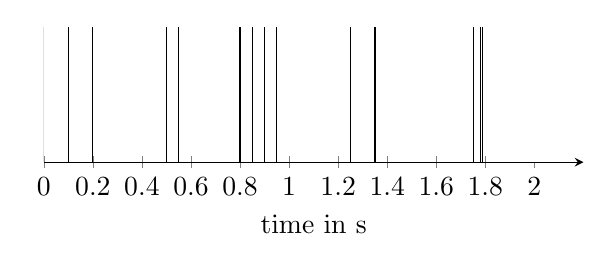
\begin{tikzpicture}
      \begin{axis}[domain=0:2, ymin=0, ymax=0.1, no markers, xtick={0,0.2,0.4,0.6,0.8,1.0,1.2,1.4,1.6,1.8,2.0}, axis x line=bottom, axis y line=none, enlargelimits=upper, y post scale=0.3, xlabel={time in s}]
        \foreach \x in {0,0.1,0.2,0.5,0.55,0.8,0.85,0.9,0.95,1.25,1.35,1.75,1.78,1.79}
          \addplot[black] coordinates{(\x,0) (\x,1)};
        \addplot[white] coordinates{(2,0) (2,1)};
      \end{axis}
    \end{tikzpicture}
    \caption{``Data'' for firing neurons: each line stands for a firing.}
    \label{fig:2014-06-30_firing_neuron_data}
  \end{subfigure}
  \begin{subfigure}{.45\textwidth}
    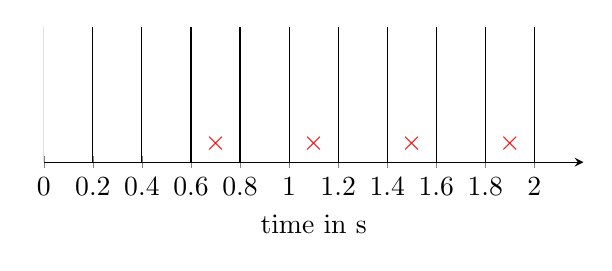
\begin{tikzpicture}
      \begin{axis}[domain=0:2, ymin=0, ymax=0.1, no markers, xtick={0,0.2,0.4,0.6,0.8,1.0,1.2,1.4,1.6,1.8,2.0}, axis x line=bottom,axis y line=none, enlargelimits=upper, y post scale=0.3, xlabel={time in s}]
        \foreach \x in {0,0.2,0.4,0.6,0.8,1.0,1.2,1.4,1.6,1.8,2.0}
          \addplot[black] coordinates{(\x,0) (\x,1)};
        \node[above,green] at (axis cs:0.1,0) {$\checkmark$};
        \node[above,green] at (axis cs:0.3,0) {$\checkmark$};
        \node[above,green] at (axis cs:0.5,0) {$\checkmark$};
        \node[above,red]   at (axis cs:0.7,0) {$\times$};
        \node[above,green] at (axis cs:0.9,0) {$\checkmark$};
        \node[above,red]   at (axis cs:1.1,0) {$\times$};
        \node[above,green] at (axis cs:1.3,0) {$\checkmark$};
        \node[above,red]   at (axis cs:1.5,0) {$\times$};
        \node[above,green] at (axis cs:1.7,0) {$\checkmark$};
        \node[above,red]   at (axis cs:1.9,0) {$\times$};
      \end{axis}
    \end{tikzpicture}
    \caption{Model for firing neurons: Bins to show whether a neuron fired during that time or not.}
    \label{fig:2014-06-30_firing_neuron_model}
  \end{subfigure}
  \caption{Example data for firing neurons and the respective model}
  \label{fig:2014-06-30_firing_neurons}
\end{figure}

We can then find the distribution over time for the neuron by taking an interval of time and counting the number of spikes. This will result in the Poisson distribution: $P(N=n|r,t)=\frac{(rt)^n}{n!}e^{rt}$.

Assuming we have 10 spikes in a second and plug this into the Poisson distribution, we should intuitively end up with 10 Hz.

\begin{align*}\index{Maximum likelihood}
P(N=n|r,t) &= \frac{(rt)^n}{n!} e^{-rt} \\
\log{P(N=n|r,t)} &= n \log{rt} - \log{n!} - rt \\
\frac{\partial\log{P(N=n|r,t)}}{\partial r} &= \frac{n}{rt}t-t \\
\frac{\partial^2\log{P(N=n|r,t)}}{\partial^2 r} &= \frac{n}{r^2} \\
\text{Use the first derivative to maximize it:}\\
\frac{n}{\est{r}t}t-t &= 1 \\
\frac{n}{\est{r}t} &= 1 \\
\frac{n}{t} &= \est{r}
\end{align*}

\subsubsection*{Bonus Question}
\begin{align*}
E(N) &= \sum_{n=0}^\infty{n \frac{(rt)^n}{n!} e^{-rt}} \\
     &= e^{-rt} \sum_{n=0}^\infty{\frac{(rt)^n}{(n-1)!}} \\
\text{use:}&\\
\sum_{n=0}^\infty{\frac{(rt)^n}{n!} e^{-rt}} &= 1 \\
\text{for:}&\\
E(N) &= e^{-rt} (rt) \sum_{n=1}^\infty{\frac{(rt)^{(n-1)}}{(n-1)!}} \\
     &= e^{-rt} (rt) \sum_{n=0}^\infty{\frac{(rt)^{n}}{n!}} \\
     &= e^{-rt} (rt) e^{rt} = rt
\end{align*}
So it's exactly what we said above: If we have 10 spikes in a second, we come up with 10 Hz.
\begin{align*}
var(N) &= E(N^2)-E(N)^2 \\
       &= \sum_{n=0}^\infty{n^2 \frac{(rt)^n}{n!} e^{-rt}} - (rt)^2 \\
       &= \sum_{n=0}^\infty{(n+1) \frac{(rt)^{n+1}}{n!} e^{-rt}} \\
       &= (rt)e^{-rt}\left[ \underbrace{ \sum_{n=0}^\infty{n \frac{(rt)^n}{n!}} }_{rt\cdot e^{rt}} +  \underbrace{ \sum_{n=0}^\infty{\frac{(rt)^n}{n!}} }_{e^{rt}} \right] - (rt)^2 \\
       &= (rt)e^{-rt}\left(rt e^{rt}+e^{rt}\right) - (rt)^2 \\
       &= (rt)(rt+1)-(rt)^2 = rt
\end{align*}
This variance corresponds with the Weber-Fechner-law (for details see \href{http://en.wikipedia.org/wiki/Weber-Fechner_law}{Wikipedia}): If the signal increases, also the noise (i.e. the variance) increases.

\subsection*{Exercise 2}
% distribution here
\begin{align*}
\frac{P(N=n|r=80 Hz, t = 100 ms)}{P(N=n|r=20 Hz, t = 100 ms)} &= \frac{ \frac{8^n}{n!}e^{-8} }{ \frac{2^n}{n!} e^{-2} } = \left(\frac{8}{2}\right)^n e^{-8+2}
\end{align*}

For the intersection we set $\left(\frac{8}{2}\right)^n e^{-8+2} = 1$.
\begin{align*}
\left(\frac{8}{2}\right)^n e^{-8+2} &= 1\\
4^n &= e^6 \\
n \log 4 &= 6 \\
n &\approx 4.3
\end{align*}

\subsection*{Exercise 3}


\subsection*{Exercise 4}


\subsection*{Exercise 5}


\end{document}
